\subsection{1d}

\lstinputlisting{p1d.py}
Next is the Kuiper test. As with the KS test, I am unsure where I went wrong
because I followed the slides but to no avail. With time constraints, 
I was not able to figure it out. Figures are plotted below. One obvious 
explanation is that my distribution does not fit a Gaussian.
I am unsure of potential (and likely) bugs in my code.
\begin{figure}[h!]
    \centering
    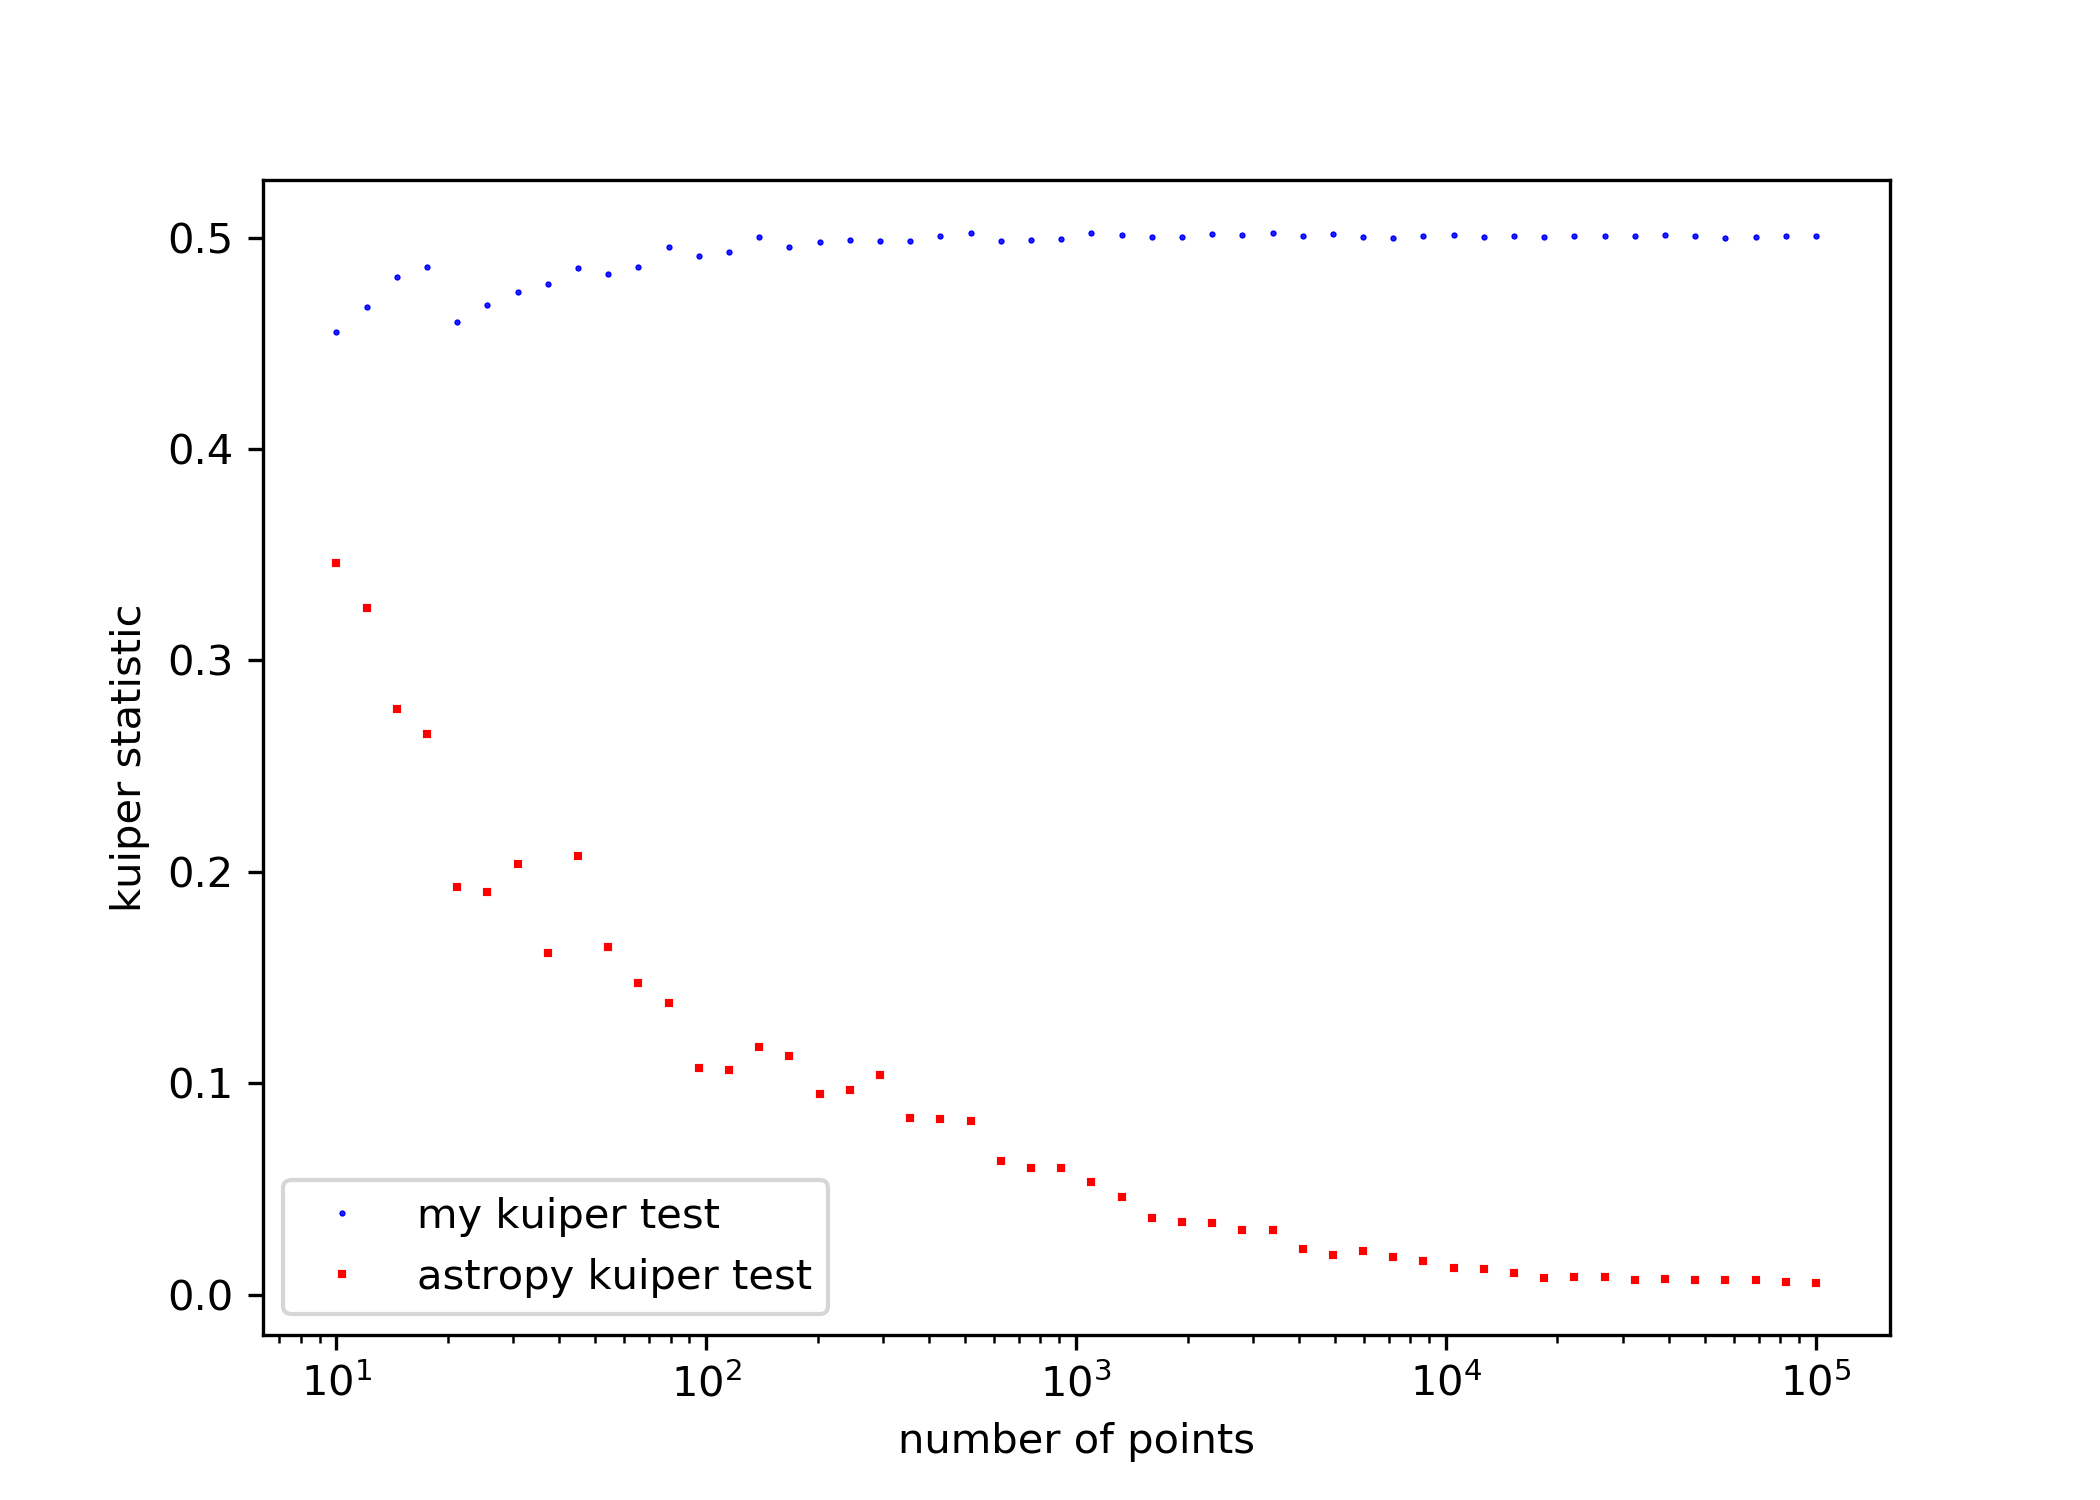
\includegraphics[width=0.9\linewidth]{./plots/kuiper_stat.png}
    \caption{Kuiper distance statistic.}
    \label{kuip_s}
\end{figure}

\begin{figure}[h!]
    \centering
    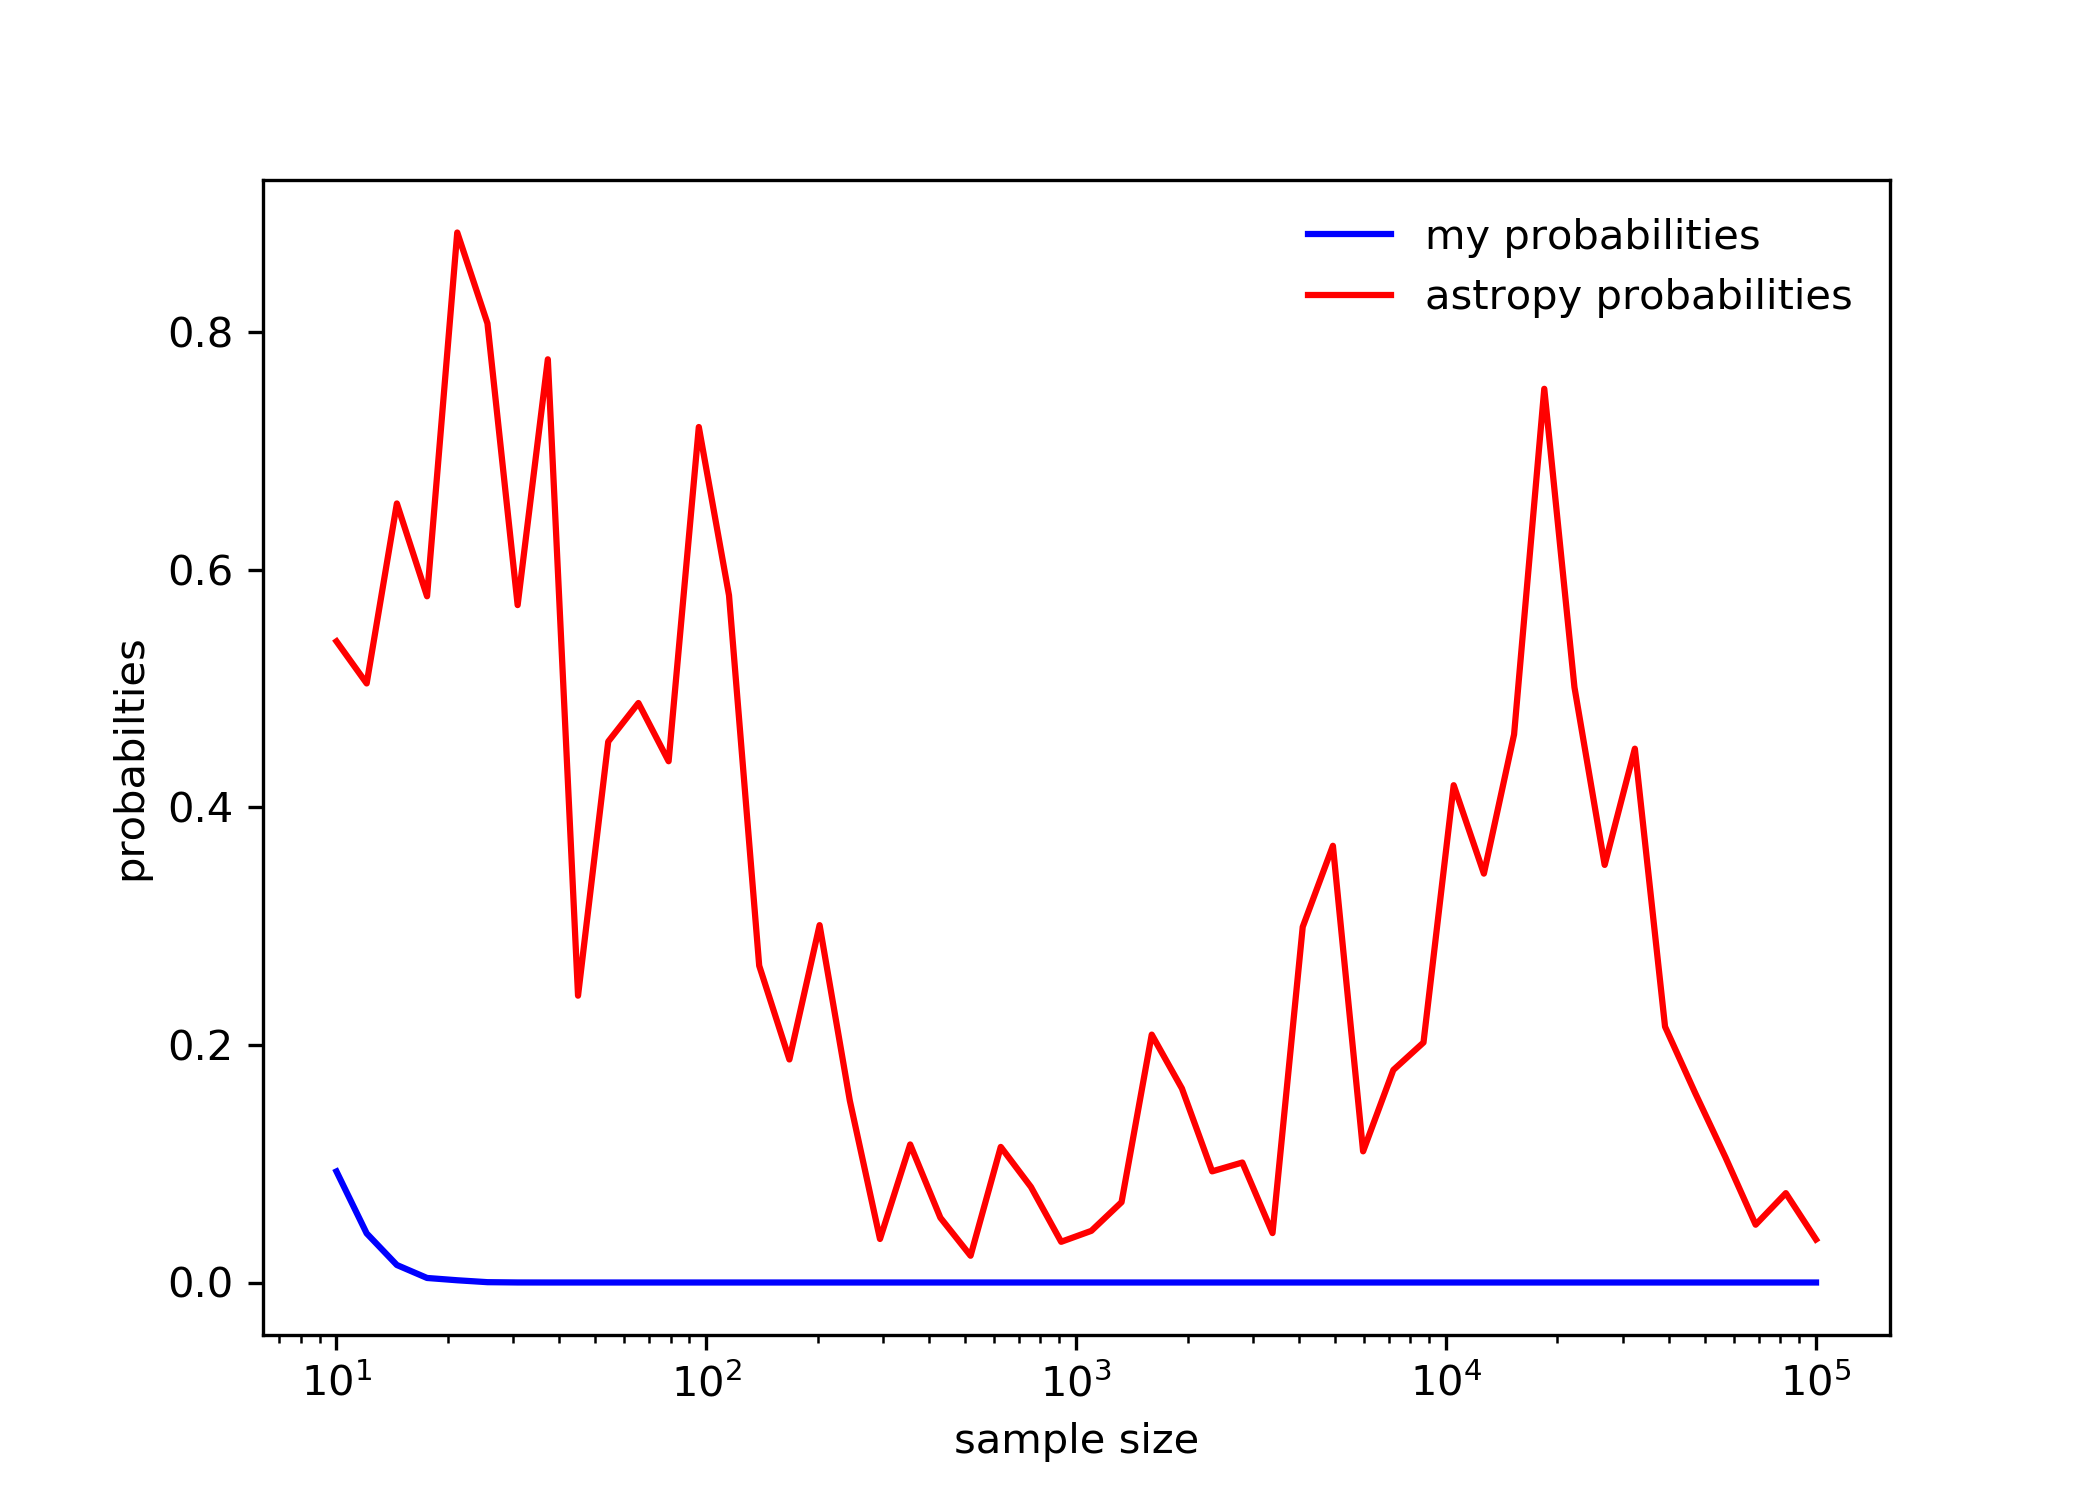
\includegraphics[width=0.9\linewidth]{./plots/k_prob.png}
    \caption{Kuiper probabilities.}
    \label{kuip_p}
\end{figure}

